\section{Mise \`a jour}
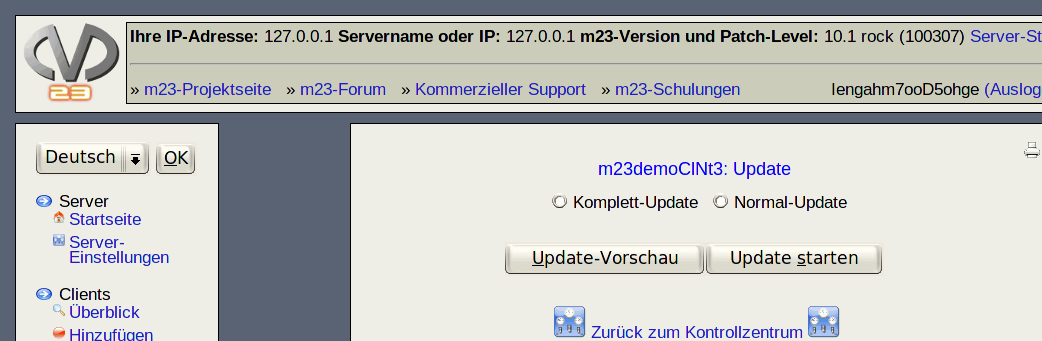
\includegraphics[scale=0.4]{/mdk/doc/manual/screenshots/fr/update_packages.png} \\
Avec la fonction de mise \`a jour, vous pouvez mettre \`a jour le logiciel sur le(s) poste(s) client. Si vous avez s\'electionn\'e un poste client singulier, vous pouvez voir une pr\'evision de la mise \`a jour.\\
\subsection{Genres de la mise \`a jour}
\begin{itemize}
\item \textbf{Mise � jour normale:} Met \`a jour les paquets install\'es et installe seulement des paquets additionels s'ils sont absolument n\'ecessaires.\\
\item \textbf{Mise � jour compl�te:} Les paquets install\'es seront mis \`a jour, des nouveaux paquets seront install\'es et des vieux paquets seront effac\'es.\\
\end{itemize}
